\documentclass{article}

\usepackage[utf8]{inputenc}

\usepackage{graphicx}
\graphicspath{{images/}}

\renewcommand{\familydefault}{\sfdefault}
\usepackage[a4paper]{geometry}

\usepackage{listings}

\usepackage{tcolorbox}
\newtcolorbox{keypointbox}
{
    arc=0mm,
    colback=red!20,
    colframe=red!80,
    leftrule=5pt,
    toprule=0pt,
    rightrule=0pt,
    bottomrule=0pt
}

\setcounter{secnumdepth}{2}

\usepackage{amsmath}
\usepackage{amssymb}
\usepackage{bm}

\newcommand{\norm}[1]{\left\lVert#1\right\rVert}

\usepackage{hyperref}
\usepackage{cleveref}

\title{Physically Based Simulation}
\author{Alexander Schlögl}

\begin{document}
\maketitle

\tableofcontents

This is \textbf{my interpretation} of the lecture slides.
I tried to be very verbose and explain everything, all while removing irrelevant parts from the lecture.
Using this you should be able to pass the lecture easily.
\large{\textbf{However, I do not take responsibility for any bad results and will not be blamed from anyone.
This was a lot of work and I did it to save others (especially students of following semesters) from having to do this themselves.
Use this summary at your own responsibility.}}
If you have any feedback, feel free to create an issue on the \href{https://github.com/alxshine/lecture-notes}{git}.
I don't promise I will fix anything, but I will try.
\newpage

\section{Introduction}
Physically based simulation is exactly what it sounds like.
Creating accurate visualizations of real world objects by simulating the underlying physical equations.
While doing so, a number of shortcuts is taken to speed up computation time.
We do not need very accurate results, we need results that \textbf{look accurate}.

\section{Mass Spring Systems}
Mass Spring Systems are a simple way of simulating deformation, and they are often used for hair, clothes etc.
The main steps of employing mass spring systems are:
\begin{enumerate}
    \item Discretizing the object into mass points and connecting them with springs
    \item Setting up the equations of motion
    \item Discretizing the equations of motion in time
    \item Determining internal and external forces acting on mass points
    \item Solving the equations numerically
\end{enumerate}

The location and mass distribution of the discretized points has a large influence on the accuracy of the simulation.
The simplest approximation is just giving all points equal mass, but better methods exist.
Each point has a position $\bm{x_i}$, a velocity $\bm{v_i}$ and a mass $\bm{m_i}$.
The points are then connected with springs.
The spring topology also heaviliy influences the accuracy, and certain heuristics exist.
Each spring stores a stiffness $k_q$, rest length $L_q$ and current length $l_q$.

\subsection{External Forces $f^{Ext}$}
External forces include gravity ($f^G_i = m_i \left[0\quad0\quad9.81\right]^T m/s^2$), friction and collisions.

\subsection{Internal Forces $f^{Int}$}
The internal forces are the forces exerted by the springs, as well as (viscous) damping.
Spring force is given by Hooke's law:
\begin{equation}
    f = k(L-l)
\end{equation}
or in 3D
\begin{equation}
    \bm{f_{ij}} = k(L-\norm{\bm{x_i} - \bm{x_j}})\frac{\bm{x_i}-\bm{x_j}}{\norm{\bm{x_i}-\bm{x_j}}}
\end{equation}
for multiple springs connected to a single mass point, just sum up all the individual spring forces.

\subsection{Spring Topologies and Parameters}
In general springs are connected in three different ways.
Structural springs connect neighboring points and oppose stretching; diagonal strings oppose shearing and interleaving springs oppose bending.
For cloth or other objects that need to be bent, springs that skip multiple points can be used.

The stiffness for the springs can be calculated with existing heuristics or be set in such a way that they accurately represent known deformations.
Usually manual tuning is required.

\subsection{Equations of Motion}
As the mass of the points, as well as the forces acting on them is known, we can simulate them using Newton's laws of motion.
From Newton's second law follows
\begin{equation}
    \label{eq:acceleration}
    m_i\frac{d^2\bm{x_i}(t)}{dt^2} = \bm{f_i^{Int}}(t) + \bm{f_i^{Ext}}(t)
\end{equation}
with which we can calculate the acceleration and update the velocity of the mass point.
\Cref{eq:acceleration} is a first order ordinary differential equation (ODE), which we can solve and the numerically integrate.
For the integration step we differentiate between explicit methods (where all required quantities are known) and implicit methods (where we need to solve a system of equations).

\subsection{Numerical Integration Methods}
As we actually need two integrations for our systems (one for $\bm{v}$ and one for $\bm{x}$) we need two seperate integration steps.
For this we simply introduce a variable for velociy and integrate it to get the new position.

All integration methods are derived from Taylor series expansion, and some use multiple Taylor series or more parts of it to reach higher accuracy.
As a reminder, the Taylor series for $y(x)$ about development point $t$ is
\begin{equation}
    y(x) = \sum_{n=0}^\infty \frac{y^{(n)}(t)}{n!} (x-t)^n
\end{equation}
and if we evaluate this at point $t+h$ we get
\begin{equation}
    \label{eq:taylor}
    y(t+h) = y(t) + y'(t)h+\frac{y''(t)}{2!}h^2 + \frac{y'''(t)}{3!}h^3+...
\end{equation}

From that we can derive our numerical integration methods and their accuracy.

\subsubsection{Euler Method}
Forward Euler is the simplest integration method.
It is derived by using the first two summands of the Taylor series, giving us the following equation
\begin{equation}
    y(t+h) = y(t) + y'(t)h + \mathcal{O}(h^2)
\end{equation}
with our error being a function in the realm of $\mathcal{O}(h^2)$.

The following calculations are done for the Forward Euler:
\begin{itemize}
    \item $\bm{x}(t+h) = \bm{x}(t) + h\cdot \bm{v}(t)$
    \item $\bm{f}(t) = \bm{f}^{Int}(t) + \bm{f}^{Ext}(t)$
    \item $\bm{a}(t) = \frac{1}{m}(\bm{f}(t)-\gamma \bm{v}(t))$ (where $\gamma$ is the damping factor)
    \item $\bm{v}(t+h) = \bm{v}(t) + h \cdot \bm{a}(t)$
\end{itemize}

In order to improve behaviour of the Euler method, we can either directly reuse new positions
\begin{align}
    \bm{x}(t+h) &= \bm{x}(t) + h \bm{v}(t)\\
    \bm{v}(t+h) &= \bm{v}(t) + h \bm{a}(\bm{x}(t+h), \bm{v}(t))
\end{align}
or directly reuse the new velocities
\begin{align}
    \bm{v}(t+h) &= \bm{v}(t) + h \bm{a}(\bm{x}(t), \bm{v}(t))\\
    \bm{x}(t+h) &= \bm{x}(t) + h \bm{v}(t+h)
\end{align}

Using these improvements is known as the Symplectic Euler.

\subsubsection{Heun's Method}
This integrator uses more summands in its approximation:
\begin{equation}
    \label{eq:heun}
    y(t+h) = y(t) + h y'(t) + \frac{h^2}{2}y''(t) + \mathcal{O}(h^3)
\end{equation}
As we don't know the second derivative, we approximate it with forward differences:
\begin{equation}
    \label{eq:second_derivative}
    y''(t) = \frac{y'(t+h) - y'(t)}{h} + \mathcal{O}(h)
\end{equation}

By plugging \Cref{eq:second_derivative} into \Cref{eq:heun} we get
\begin{align}
    y(t+h)  &\approx y(t) + hy'(t) + \frac{h^2}{2} (\frac{y'(t+h)-y'(t)}{h})\\
            &\approx y(t) + hy'(t) + \frac{h}{2} y'(t+h) - \frac{h}{2} y'(t)\\
            &\approx y(t) + \frac{h}{2}(y'(t) + y'(t+h))
\end{align}

As we don't know $y'(t+h)$ yet when we evaluate this, we approximate it with a regular Euler step.

\begin{keypointbox}
    Heun's method uses the average of the current velocity and the next velocity for the update step
\end{keypointbox}

The implementation steps for Heun's method are the following
\begin{itemize}
    \item $\bm{a}(t) = \frac{1}{m}(\bm{f}(t) - \gamma \bm{v}(t))$
    \item $\bm{\tilde{v}}(t+h) = \bm{v}(t) + h\bm{a}(t)$
    \item $\bm{\tilde{x}}(t+h) = \bm{x}(t) + h\bm{\tilde{v}}(t)$
    \item $\bm{\tilde{a}}(t+h) = \frac{1}{m}(\bm{\tilde{f}}(t+h) - \gamma \bm{\tilde{v}}(t+h))$
    \item $\bm{x}(t+h) = \bm{x}(t) + h \frac{\bm{v}(t) + \bm{\tilde{v}}(t+h)}{2}$
    \item $\bm{v}(t+h) = \bm{v}(t) + h \frac{\bm{a}(t) + \bm{\tilde{v}}(t+h)}{2}$
\end{itemize}

\subsubsection{Midpoint Method}
Heun's method averages $y'(t)$ and $y'(t+h)$.
The midpoint method only determinse $y'$ at $t+h/2$, giving us the same accuracy with less work.
We approximate $y'(t+h/2)$ with an Euler step.

For our mass spring use case we need to approximate both $\bm{\tilde{v}}$ and $\bm{\tilde{a}}$ (and thus $\bm{\tilde{x}}$) for $t+h/2$.

\subsubsection{Runge-Kutta Methods}
These are more general cases of the Midpoint method.
They increase accuracy by performing intermediate steps.
The most common variant is RK4.
Due to the increased accuracy, larger timesteps can be used, but this increases computational overhead.

RK4 works as follows:
\begin{align}
    k_1 &= f(t, y(t))\\
    k_2 &= f(t+h/2, y(t)+h/2k_1)\\
    k_3 &= f(t+h/2, y(t)+h/2k_2)\\
    k_4 &= f(t, y(t)+hk_3)
\end{align}
The value for $y(t+h)$ is the calculated using a weighted average
\begin{equation}
    y(t+h) = y(t) + \frac{h}{6} (k_1 + 2k_2 + 2k_3 + k_4)
\end{equation}

Implementation of RK4 (or any RK method) should be pretty clear.

\subsubsection{Verlet Method}
For this method we start with two Taylor series expansions:
\begin{align}
    y(t+h) &= y(t) + y'(t)h + \frac{y''(t)}{2!}h^2 + \frac{y'''(t)}{3!}h^3 + \mathcal{O}(h^4)\\
    y(t-h) &= y(t) - y'(t)h + \frac{y''(t)}{2!}h^2 - \frac{y'''(t)}{3!}h^3 + \mathcal{O}(h^4)
\end{align}
then, by summing them up we get
\begin{equation}
    y(t+h) = 2y(t) - y(t-h) + h^2y''(t) + \mathcal{O}(h^4)
\end{equation}

As you can see the velocity terms cancels out, leading to the typical assumption that the force term is independent of velocity (no damping).
The Verlet method is a symplectic integrator (it has nice energy conservation properties in Hamiltonian systems) and is also time reversible.

The velocity term here is never explicitly calculated.
If we do need it (e.g. for kinetic energy) we need to approximate it either via backward or central differences.

\subsubsection{Leapfrog Method}
The main goal of this method is to improve the velocity estimate.
It is similar to the Verlet method but from the Taylor series for velocity:
\begin{align}
    \bm{v}(t+h) &= \bm{v}(t) + \bm{v}'(t)h + \frac{\bm{v}''(t)}{2!}h^2 + \frac{\bm{v}'''(t)}{3!} h^3 + \mathcal{O}(h^4)\\
    \bm{v}(t-h) &= \bm{v}(t) - \bm{v}'(t)h + \frac{\bm{v}''(t)}{2!}h^2 - \frac{\bm{v}'''(t)}{3!} h^3 + \mathcal{O}(h^4)
\end{align}
and by subtracting we get
\begin{equation}
    \bm{v}(t+h) = \bm{v}(t-h) + 2\bm{v}'(t)h + \mathcal{O}(h^3)
\end{equation}

The Leapfrog method then employs shifted updates, with $\bm{v}$ being updated for $t+h/2$ and $\bm{x}$ and $\bm{a}$ being updated for $t$.
This gives us an error of only $\mathcal{O}(h^3)$ with only one force evaluation.
We need to initialize $\bm{v}(t_{1/2})$ with e.g. an Euler step.

\subsubsection{Implicit Euler}
The Implicit Euler formulates the update equation like as follows
\begin{equation}
    y_{n+1} = y_n + h \cdot f(t_{n+1}, y_{n+1})
\end{equation}

Due to this, we have to solve for an unknown in every update step.
One option is the \textbf{fixed-point iteration}
\begin{equation}
    y_{n+1}^{(k+1)} = y_n + h \cdot f(t_{n+1}, y_{n+1}^{(k)})
\end{equation}
which requires initialization such as $y_{n+1}^{(0)} = y_n$ or $y_{n+1}^{(0)} = y_n + h \cdot f(t_n, y_n)$.

Another option would be \textbf{Newton's Method}.

\subsection{Test Equation}
We can study stability behaviour of a solver via a linear test equation (Dahlquist's equation):
\begin{equation}
    \label{eq:dahlquist}
    y'(t) = \lambda \cdot y(t)
\end{equation}
which gives us the following solution for $y(t)$ (assuming $\lambda \in \mathbb{R}$)
\begin{equation}
    y(t) = e^{\lambda t} y_0
\end{equation}

An example for the forward Euler:
The update step is
\begin{equation}
    y_{n+1} = y_n + h \cdot y_n'
\end{equation}
by inserting the test equation we get
\begin{equation}
    y_{n+1} = (1 + \lambda h) y_n
\end{equation}
which with recursive evaluation gives us
\begin{equation}
    y_{n+1} = (1 + \lambda h)^{n+1} y_0
\end{equation}

This shows that the forward Euler is unconditionally unstabel if $\lambda > 0$ and stable iff $-2 < h\lambda < 0$.

\subsection{Collision Handling}
When using mass spring systems, a simple form of collision detection and handling can be required.
For this, penalty forces are used.
In the penalty forces approach any penetration of an object into another creates a spring force separating both objects.
This approach is only an approximation, but can be very useful due to its simplicity.

\subsection{Problems of Mass Spring Systems}
The behaviour of the system is topology dependent.
Also, we do not have an explicit notion of volume preservation, which can result in systems collapsing on themselves.
This is again dependent on their topology.

\section{Solving PDEs with Finite Elements}
Differential equations relate an unknown functions with its derivatives.
They are typically employed to describe physical laws and phenomena, e.g. growth or decay.

\subsection{Types of Differential Equations}
\subsubsection{Ordinary Differential Equations (ODEs)}
These describe an unknown function only based on derivatives with respect to a single varible.

\subsubsection{Partial Differential Equations (PDEs)}
Describe an unknown function based on its derivatives with respect to multiple variables.
The \textbf{order} $n$ of a PDE is given by its highest derivative.
PDEs are called linear if the coefficients of the function and the derivatives are independent of the latter (e.g. no multiplication between them).

\subsubsection{Classification of Second Order PDEs}
Physical phenomena are often modeled as second order linear PDEs of the form
\begin{equation}
    a \cdot u_{xx} + b \cdot u_{xy} + c \cdot u_{x} + e \cdot u_{y} + k \cdot u = g(x,y)
\end{equation}

Then, based on the coefficients we differentiate three classes:
\begin{itemize}
    \item \textbf{Hyperbolic:} $b^2 - 4ac > 0$
    \item \textbf{Parabolic:} $b^2 - 4ac = 0$
    \item \textbf{Elliptic:} $b^2 - 4ac < 0$
\end{itemize}

\subsection{Initial and Boundary Conditions}
In order to find a specific solution to the PDE we need to have some value to start from.
This can be either done by \textbf{initial conditions}, which specify a certain physical state at start time, or \textbf{boundary conditions}, which impose a state on the boundary $\delta \Omega$ of the solution domain $\Omega$.

\subsection{Solving PDEs}
Unfortunately, closed form analytical solutions exist only for very simple problems.
This makes numerical analysis in order to get an approximate solution necessary.
Typical solution methods are \textbf{finite differences} and \textbf{finite elements}.
Only the finite element method is described in the lecture slides.

\subsection{Finite Element Method}
The key idea is to divide the domain into many small elements and then approximate the true solution in each element via a set of simple equations.
After the individual equations are solved, they are combined into a global system for the final solution for the given boundary conditions.

\subsubsection{Piecewise Approximation}
In order to make the numerical solving easier, we approximate the target function via a linear combination of basis functions.
Given a set of discrete evaluations of the function $f$, we want to find a way to get the values between those points for a continuous evaluation.
As linear interpolation is a very intuitive form of doing so, we want a simple way of calculating this.
This is done via "hat" functions, which can be seen in \Cref{fig:hat}.

\begin{figure}[h]
    \centering
    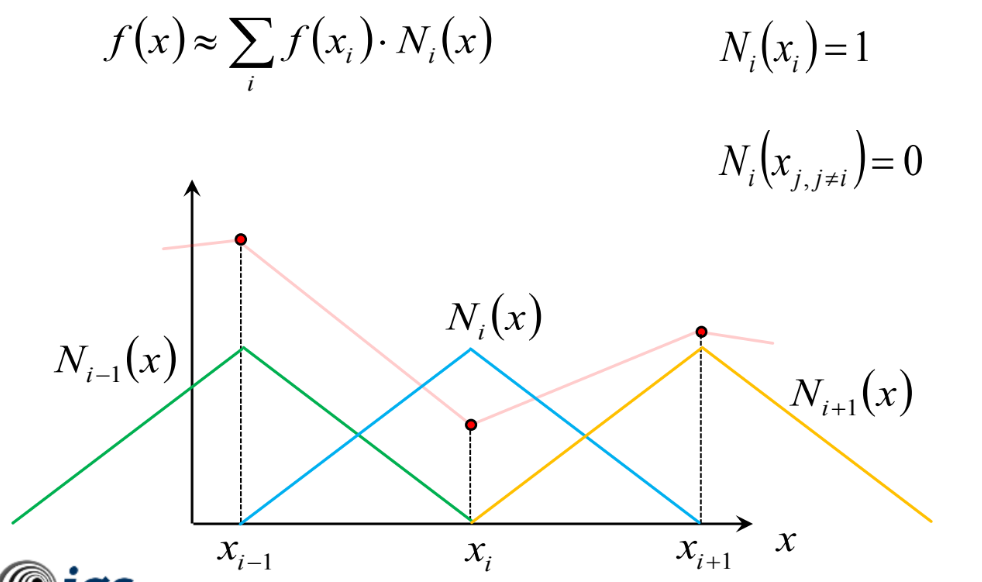
\includegraphics[width=0.9\textwidth]{hat.png}
    \caption{An example of interpolation via hat functions}
    \label{fig:hat}
\end{figure}

For the finite element method we utilize the Ritz-Galerkin approach, which approximates the true solution with a linear combination of basis functions:
\begin{equation}
    u \approx \sum_i u_i \cdot N_i
\end{equation}
with unknowns $u_i$.
We then select an arbitrary test function as linear combination of the basis functions
\begin{equation}
    v \approx \sum_j N_j
\end{equation}
which gives us the following approximations of the derivatives
\begin{equation}
    \nabla u \approx \sum_i u_i \cdot \nabla N_i \qquad \nabla v \approx \sum_j \nabla N_j
\end{equation}


\subsubsection{Derivation of the Element Equation}
We start from the 2D Poisson equation on a domain $\Omega$ with Dirichlet boundary conditions (a fixed value on the domain boundary)
\begin{equation}
    \label{eq:poisson}
    \Delta u(x,y) = f(x,y), \qquad u(x,y) = 0 \textup{ for } (x,y) \in \delta \Omega
\end{equation}
Then we multiply with a sufficiently smooth (differentiable twice)  test function $v(x,y)$ with $v(x,y)=0$ on boundary $\delta \Omega$.
\begin{equation}
    \Delta u(x,y) v(x,y) = f(x,y) v(x,y)
\end{equation}
This we integrate over the domain
\begin{equation}
    \int_\Omega \Delta u(x,y) v(x,y) d\Omega = \int_\Omega f(x,y) v(x,y) d\Omega
\end{equation}

Then we derive the \textbf{weak form} of the problem by applying the Green-Gauss theorem (similar to integrating by parts)
\begin{equation}
    \int_\Omega \nabla u(x,y) \nabla v(x,y) d\Omega = \int_\Omega f(x,y) v(x,y) d\Omega
\end{equation}

After inserting the Ritz-Galerkin approxmation into the weak form we get
\begin{align}
    \int_\Omega \sum_i u_i \cdot \nabla N_i \cdot \sum_j \nabla N_j d\Omega &= \int_\Omega f \cdot \sum_j N_j d\Omega\\
    \sum_i u_i \int_\Omega \nabla N_i \cdot \sum_j \nabla N_j d\Omega &= \int_\Omega f \cdot \sum_j N_j d\Omega
\end{align}
and by splitting this into a set of single equations we get
\begin{equation}
    \sum_i u_i \int_\Omega \nabla N_i \cdot \nabla N_j d\Omega = \int_\Omega f \cdot N_j d\Omega \qquad \forall j=1,...,n
\end{equation}

We can write this system of equations as a matrix, which is symmetric, positive definite and banded.
The so called \textbf{stiffness matrix} $K$ can be solved with an iterative solver, e.g. conjugate gradient method.
Due to the sparsity of the stiffness matrix it is easiest assembled element-wise.

\subsubsection{Linear Triangulation}
In 2D we want our linear tringular elements to be composed of three nodes with three linear basis functions:
\begin{equation}
    N_i(x,y) = c_{i,0} + c_{i,1} x + c_{i,2}y \qquad i=1,2,3
\end{equation}
It is important to note that these basis functions have local support, ie. they are only non-zero for adjacent points.

\subsubsection{Assembling the Stiffness Matrix}
We want to evaluate the following equations
\begin{align}
    K_{ij} &= \int_\Omega \nabla N_i \cdot \nabla N_j d\Omega\\
    K_{ij} &= \int_\Omega (\frac{\partial N_i}{\partial x}, \frac{\partial N_i}{\partial y}) \cdot (\frac{\partial N_j}{\partial x}, \frac{\partial N_j}{\partial y}) dxdy\\
    K_{ij} &= \int_\Omega \frac{\partial N_i}{\partial x} \cdot \frac{\partial N_j}{\partial x} + \frac{\partial N_i}{\partial y} \cdot \frac{\partial N_j}{\partial y} dxdy
\end{align}
The basis function $N_i$ extends over all elements adjacent to node $i$ and is zero outside of $\Omega_i$.
$K_ij \neq 0$ if there exists an element (triangle) containing nodes $i$ and $j$.

\subsubsection{Right-Hand Side}
We assemble the right hand side with similar assumptions as before:
\begin{equation}
    f_j = \sum_{\textup{adjacent}} \int_{\Omega_e} f \cdot N_j d\Omega_e
\end{equation}

We can approximate the integral with a one point quadrature
\begin{equation}
    \int_{\Omega_e} f \cdot N_j d\Omega_e \approx A_e \cdot f(x_c, y_c) \cdot N_j(x_c, y_c)
\end{equation}
at barycenter $(x_c, y_c)$ in order to save computation time.

\Cref{fig:stiffness} shows an example of a system setup.

\begin{figure}[h]
    \centering
    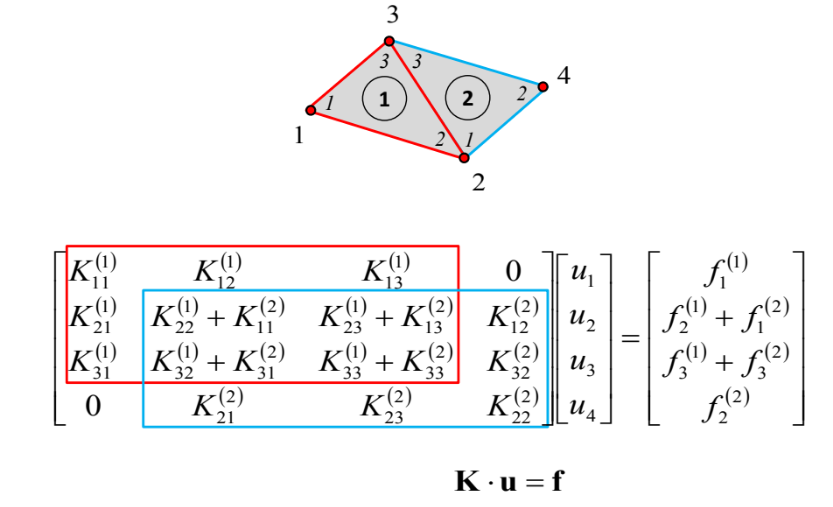
\includegraphics[width=\textwidth]{stiffness.png}
    \caption{Example setup}
    \label{fig:stiffness}
\end{figure}

\section{Solving Systems of Equations}
For calculating numerical solutions for our FEM systems we need an efficient way of solving systems of equations.
These equations can be written as $\bm{Ax} = \bm{b}$.
We could solve this by inverting the coefficient matrix $\bm{A}$, but that takes too long ($\mathcal{O}(n^3)$).
To this end we use iterative solvers, which work more efficiently.

\subsection{Jacobi Method}
The Jacobi method only converges for diagonally dominant system matrices, but this is usually a given in physical applications.
The basic approach of it is rearranging the individual equations:
\begin{gather}
    \sum_{j=1}^n a_{ij} x_j = b_i\\
    x_i = \frac{1}{a_{ii}}(b_i - \sum_{j=1, j \neq i}^{n} a_{ij} x_j)
\end{gather}
From this we derive our update rule
\begin{equation}
    x_i^{(k+1)} = \frac{1}{a_{ii}} (b_i - \sum_{j=1, j \neq i}^n a_{ij} x_j^{(k)})
\end{equation}
or in matrix notation
\begin{equation}
    \bm{x}^{(k+1)} = \bm{D^{-1} (b - (A-D)x^{(k)})}
\end{equation}

\subsection{Solving an Equivalent Problem}
This method is especially effective for sparse matrices, and requires that the matrix $\bm{A}$ be symmetric fulfill
\begin{equation}
    \bm{x}^T \bm{Ax} > 0 \qquad \forall \bm{x} \neq \bm{0}
\end{equation}

The method is then based on solving an equivalent problem, minimizing the function
\begin{equation}
    f(\bm{x}) = \frac{1}{2} \bm{x}^T \bm{Ax} - \bm{x}^T \bm{b}
\end{equation}
The first and second derivatives of the function are then
\begin{equation}
    \nabla f(\bm{x}) = \bm{Ax} - \bm{b}, \qquad \nabla^2f(\bm{x}) = \bm{A}
\end{equation}
The function $f$ is a parabola with a single global minimum.
This global minimum contains our solution, because there $\bm{Ax^*} - \bm{b} = 0$, so finding $x^*$ equals finding our solution.
We try to find the solution via line searching.

Our iteration step is
\begin{equation}
    \bm{x}^{(k+1)} = \bm{x}^{(k)} + \alpha^{(k)} \bm{p}^{(k)}
\end{equation}
with initial guess $\bm{x}^{(0)}$, search direction $\bm{p}^{(k)}$ and step length $\alpha^{(k)}$.
The question now is how to find the most efficient search direction and step length.
We approximate the error in each step $\bm{e}^{(k)} = \bm{x}^* - \bm{x}^{(k)}$ with the residual of our approximation of the right-hand side
\begin{equation}
    \bm{r}^{(k)} = \bm{b} - \bm{Ax}^{(k)} \qquad \rightarrow \bm{r}^{(k)} = -\nabla f(\bm{x}^{(k)})
\end{equation}
One can also note that $\bm{r}^{(k)} = \bm{Ae}^{(k)}$.

\subsubsection{Steepest Gradient Method}
The gradient determines the direction of greatest increase, so we step into the direction of the negative gradient
\begin{gather}
    \bm{x}^{(k+1)} = \bm{x}^{(k)} + \alpha^{(k)}\bm{p}^{(k)}\\
    \bm{p}^{(k)} = -\nabla f(\bm{x}^{(k)}) = \bm{r}^{(k)} = \bm{b} - \bm{Ax}^{(k)}
\end{gather}

We find the step size $\alpha$ by minimzing the next function value, which gives us the following formula for $\alpha$
\begin{equation}
    \alpha^{(k)} = \frac{(\bm{r}^{(k)})^T \bm{r}^{(k)}}{(\bm{r}^{(k)})^T \bm{Ar}^{(k)}}
\end{equation}
If the matrix $\bm{A}$ is ill-conditioned, this method is slow converging.
A better way of finding a search direction is needed.

\subsubsection{Conjugate Gradient Method}
The key idea here is to select a number of $\bm{A}$-conjugate directions in which to go.
Two non-zero vectors are conjugate with respect to a matrix $\bm{A}$ if $\bm{p}_i^T \bm{Ap}_j = 0$ with $\bm{p}_i \neq \bm{p}_j$.
Instead of picking a set of vectors in the beginning, we pick a new one each iteration.
\begin{equation}
    \bm{p}^{(k+1)} = \bm{r}^{(k+1)} + \beta^{(k+1)} \bm{p}^{(k)}, \qquad \bm{p}^{(0)} = \bm{r}^{(0)}
\end{equation}
Obtaining $\beta$ works as follows:
\begin{gather}
    (\bm{p}^{(k+1)})^T \bm{Ap}^{(k)} = 0\\
    (\bm{r}^{(k+1)} + \beta^{(k+1)} \bm{p}^{(k)})^T \bm{Ap}^{(k)} = 0\\
    (\bm{r}^{(k+1)})^T \bm{Ap}^{(k)} + \beta^{(k+1)} (\bm{p}^{(k)})^T \bm{Ap}^{(k)} = 0\\
    \beta^{(k+1)} = - \frac{(\bm{r}^{(k+1)})^T \bm{Ap}^{(k)}}{(\bm{p}^{(k)})^T \bm{Ap}^{(k)}}
\end{gather}

From the update method
\begin{equation}
    \bm{x}^{(k+1)} = \bm{x}^{(k)} + \alpha^{(k)} \bm{p}^{(k)}
\end{equation}
we get the equation for updating the residual
\begin{gather}
    \bm{Ax}^{(k+1)} - \bm{b} = \bm{Ax}^{(k)} - \bm{b} + \alpha^{(k)} \bm{Ap}^{(k)}\\
    \bm{r}^{(k+1)} = \bm{r}^{(k)} - \alpha^{(k)} \bm{Ap}^{(k)}\\
    \label{eq:equivalency}
    \bm{Ap}^{(k)} = \frac{\bm{r}^{(k)} - \bm{r}^{(k+1)}}{\alpha^{(k)}}
\end{gather}
\Cref{eq:equivalency} gives us another way of calculating $\beta$
\begin{equation}
    \beta^{(k+1)} = - \frac{(\bm{r}^{(k+1)})^T \bm{Ap}^{(k)}}{(\bm{p}^{(k)})^T \bm{Ap}^{(k)}} = \frac{(\bm{r}^{(k+1)})^T \bm{r}^{(k+1)}}{(\bm{r}^{(k)})^T \bm{r}^{(k)}}
\end{equation}

The step length $\alpha$ is determined by
\begin{gather}
    (\bm{r}^{(k+1)})^T \bm{r}^{(k)} = 0\\
    (\bm{r}^{(k)} - \alpha^{(k)}\bm{Ap}^{(k)})^T \bm{r}^{(k)} = 0\\
    (\bm{r}^{(k)})^T\bm{r}^{(k)} - \alpha^{(k)} (\bm{Ap}^{(k)})^T \bm{r}^{(k)} = 0\\
    \alpha^{(k)} = \frac{(\bm{r}^{(k)})^T \bm{r}^{(k)}} {(\bm{p}^{(k)})^T \bm{A}^T \bm{p}^{(k)}}
\end{gather}

\paragraph{Summary}
The iteration variables are calculated as follows:
\begin{align}
    \alpha^{(k)} &= \frac{(\bm{r}^{(k)})^T \bm{r}^{(k)}} {(\bm{p}^{(k)})^T \bm{Ap}^{(k)}}\\
    \bm{x}^{(k+1)} &= \bm{x}^{(k)} + \alpha^{(k)} \bm{p}^{(k)}\\
    \bm{r}^{(k+1)} &= \bm{r}^{(k)} - \alpha^{(k)} \bm{Ap}^{(k)}\\
    \beta^{(k+1)} &= \frac{(\bm{r}^{(k+1)})^T \bm{r}^{(k+1)}} {(\bm{r}^{(k)})^T \bm{r}^{(k)}}\\
    \bm{p}^{(k+1)} &= \bm{r}^{(k+1)} + \beta^{(k+1)} \bm{p}^{(k)}
\end{align}

We are guaranteed to find a solution after $n$ steps for an $n \times n$ matrix, but can get reasonable approximations before that.
In order to increase performance, one can use a precondition matrix $\bm{M}^{-1}\bm{Ax} = \bm{M}^{-1}\bm{b}$.
The simplest choice is using the diagonal entries of $\bm{A}$ (Jacobi preconditioner).

\subsection{FEM summary}
The required steps for FEM are
\begin{enumerate}
    \item Discretization of the domain
    \item Construction of approximate solution over elements
    \item Assembling elements into a global system
    \item Imposing boundary conditions
    \item Numerical solution of resulting equation system
    \item Post-processing and visualization of results
\end{enumerate}

FEM is widely applicable, easy to use for complex geometries, easy to adapt for better approximation and it is easy to impose boundary conditions.
However, the solution is only an approximate, careful setup is required, the amount of pre-processing required can become large, and parallelization is not straight forward (due to the interdependencies between elements).
\end{document}
